% Asset ID: AS1VectorsTikZ-003
% Asset type: TikZ diagram
% Suggested file: tikz/AS1VectorsTikZ-003_vector_addition.tex
% Source: CCEA AS1-VEC-LO003; Phase 1 Core Theory 5
% Related lesson section: Vector addition, subtraction and scalar multiplication
% Purpose: Show the triangle law of vector addition.
% Boundary note: 2D vectors only.

\documentclass[tikz,border=8pt]{standalone}
\usepackage{amsmath}
\usetikzlibrary{arrows.meta}
\begin{document}
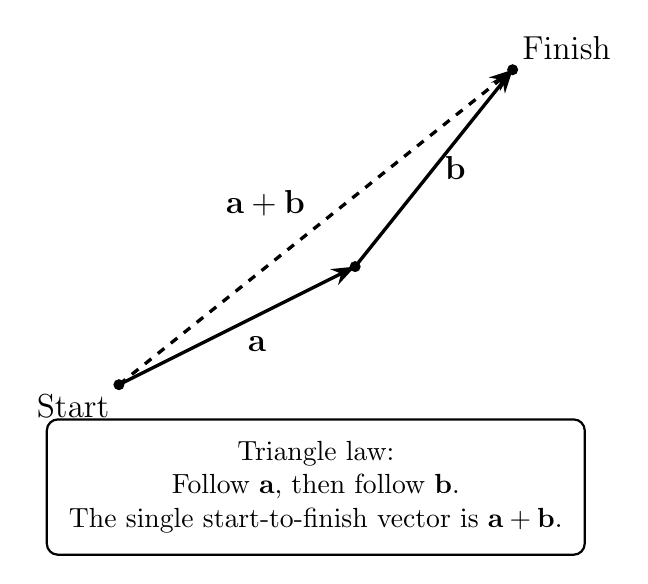
\begin{tikzpicture}[>=Stealth,vector/.style={->, very thick},resultant/.style={->, very thick, dashed},label/.style={font=\large},note/.style={draw, rounded corners, thick, align=center, inner sep=8pt}]
\coordinate (A) at (0,0); \coordinate (B) at (3,1.5); \coordinate (C) at (5,4);
\draw[vector] (A) -- (B) node[midway, below right,label] {$\mathbf{a}$};
\draw[vector] (B) -- (C) node[midway, right,label] {$\mathbf{b}$};
\draw[resultant] (A) -- (C) node[midway, above left,label] {$\mathbf{a}+\mathbf{b}$};
\fill (A) circle (2pt) node[below left,label] {Start}; \fill (B) circle (2pt); \fill (C) circle (2pt) node[above right,label] {Finish};
\node[note] at (2.5,-1.3) {Triangle law:\\ Follow $\mathbf{a}$, then follow $\mathbf{b}$.\\ The single start-to-finish vector is $\mathbf{a}+\mathbf{b}$.};
\end{tikzpicture}
\end{document}
